%\section{Verifying the experimental results}

%The second setup used for verifying the results was more simple. Only a resolver was connected to a loadless servmotor. This eliminates many of the previous potential error sources, thus making the verification results more reliable.

%The servomotor in second setup was not connected to any load. Hence, only no-load tests were possible. However, various speeds were tested when verifying the results to provide additional information.

\subsection{Cogging torque compensation}
A PM servomotor was used to verify that compensation works with different motors. The servomotor is known to have high cogging torque, which makes it ideal for testing, as this reflects typical use case for compensators. The servomotor was not connected to any load. Hence, many potential error sources were eliminated, but at the same time, only no-load tests were possible. A resolver was used for measuring speed pulsations. The servomotor parameters are listed in Table \ref{Tbl:SDM251}.
%In order to make this chapter more informative, additional tests were performed while also verifying that compensators can reduce also the servomotor pulsations. Compensation was tested in various low speeds and different speed filtering time constants were tested with ILC.

%  Due to high cogging torque, it can be expected that the sixth harmonic is high and it should get reduced significantly.
\begin{table}[ht]
\caption{SDM251 servomotor nameplate values}
\centering
\begin{tabular}[t]{lcccc}
\hline
Description & Symbol & Value & Unit\\
\hline
Nominal current (rms)  & $I_N$       & 1.5   & A\\
Nominal voltage (rms, line-line) & $U_N$       & 330.0 & V\\
Nominal frequency & $f_N$       & 150.0 & Hz\\
Nominal speed     & $\omega_N$  & 3000  & rpm\\
Nominal power     & $P_N$       & 0.72  & kW\\
Nominal torque    & $T_N$       & 2.30  & Nm\\
Number of poles   & $N_p$       & 6     & \\
\hline
\label{Tbl:SDM251}
\end{tabular}
\end{table}%


At $60$ rpm speed, the pulsations were noticeable and it was possible to hear the motor having troubles rotating smoothly due to high cogging torque. However, when compensation was enabled, the uneven noise disappeared and the motor was clearly able to keep more constant speed. The SRF measure with conventional PI control was $2.31\%$. ILC reduced SRF to $0.68\%$ and Q-learning based approach to $0.62\%$. The effects of compensation can be observed from Figs. \ref{fig:ilc-on-off} and \ref{fig:qlr-off-on} that show measured shaft speed.
\begin{figure}[b] 
    \centering
    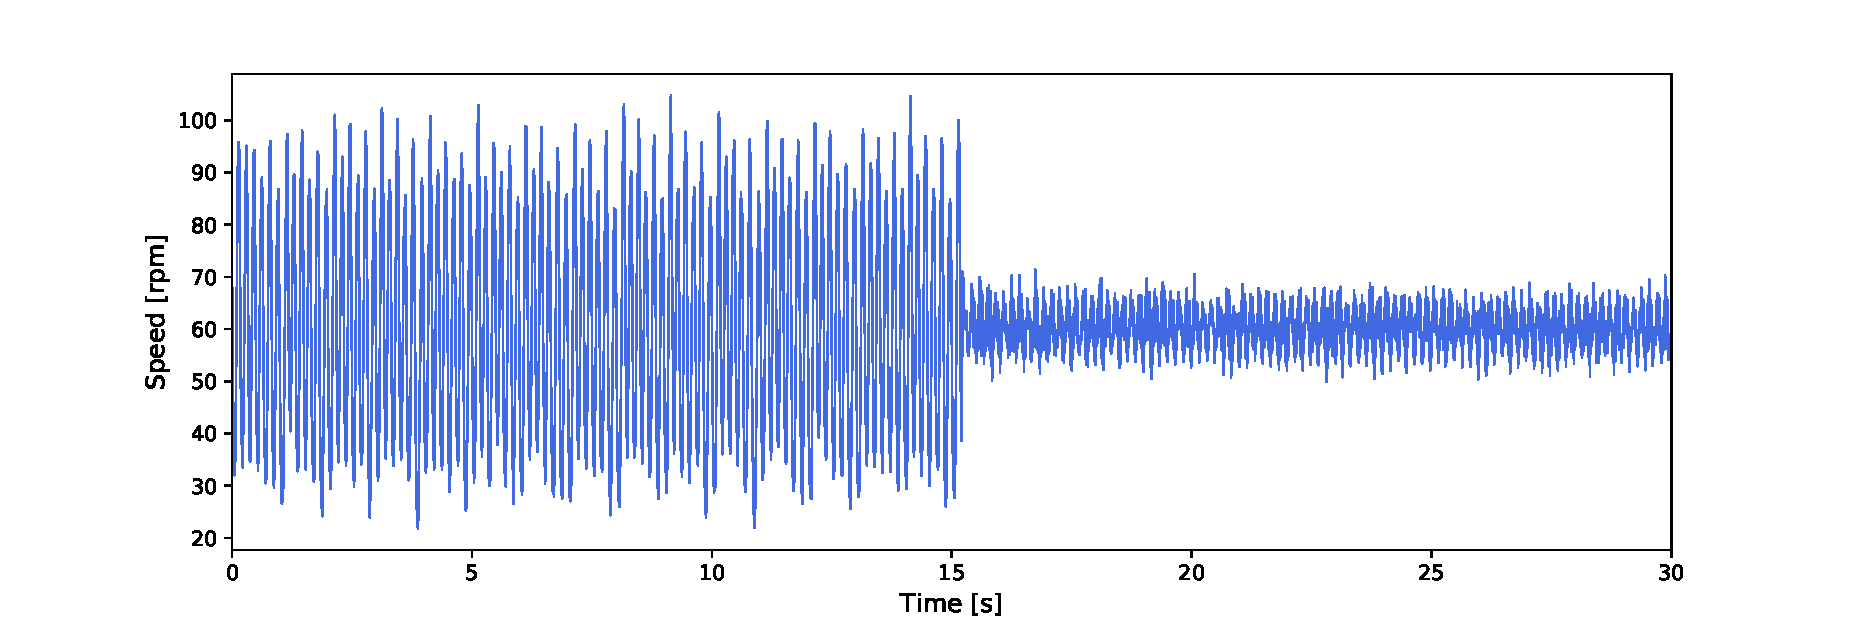
\includegraphics[width=\textwidth]{images/ILC-SDM251-OFF-ON.pdf}
    \caption{Speed ripple getting reduced when ILC based compensator is enabled}
    \label{fig:ilc-on-off}
\end{figure}
When compensators have been trained and compensation values have been saved into memory, the compensation is instantaneous with both methods. ILC appears to be more graceful for the control than Q-learning method when compensators are suddenly enabled, as it takes a few seconds for the system to stabilize with the Q-learning method. The produced waveform is also different between the methods.
\begin{figure}[tb] 
    \centering
    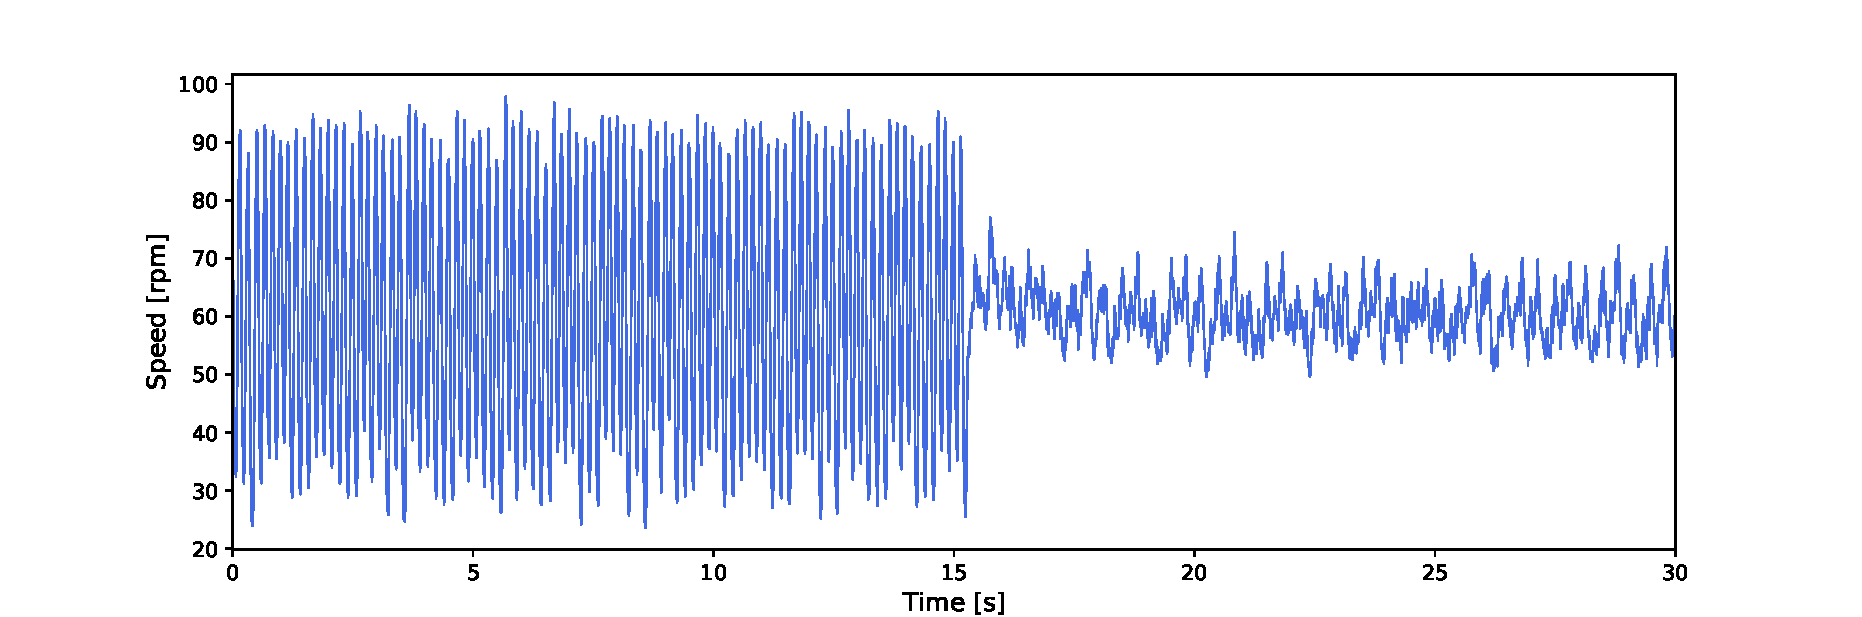
\includegraphics[width=\textwidth]{images/QLR-SDM251-OFF-ON.pdf}
    \caption{Speed ripple getting reduced when Q-learning based compensator is enabled}
    \label{fig:qlr-off-on}
\end{figure}

The ILC parameters used in the experiment, were $\Phi = 1.5$, $\Gamma = 0.9$ and $ \alpha = 0.15$. These values were experimentally found to produce best results. With Q-learning, $T_{max} = 0.03$ was used in addition to parameters values given in Table \ref{Tbl:Q-params}.

\subsection{Compensation with noisy systems}
The negative effects of noise can be reduced with filtering or by utilizing the forgetting factor with ILC. It was found that the forgetting factor is superior compared to filtering of the speed signal. This was expected result as filtering leads to phase shift, which results to delayed compensation. In the worst case, it is possible to align the compensation crests with the disturbance crests, which creates constructive inference that transforms the compensator to a disturbance amplifier. The negative effects of the filtering can be seen in Fig. \ref{Fig:ILC-filtering} where the same setup, with the same ILC gains, was run by using three different speed filtering coefficients. It can be observed that the performance is best when the speed signal is not filtered at all. Hence, filtering should be avoided. 
\begin{figure}[htb] 
    \centering
    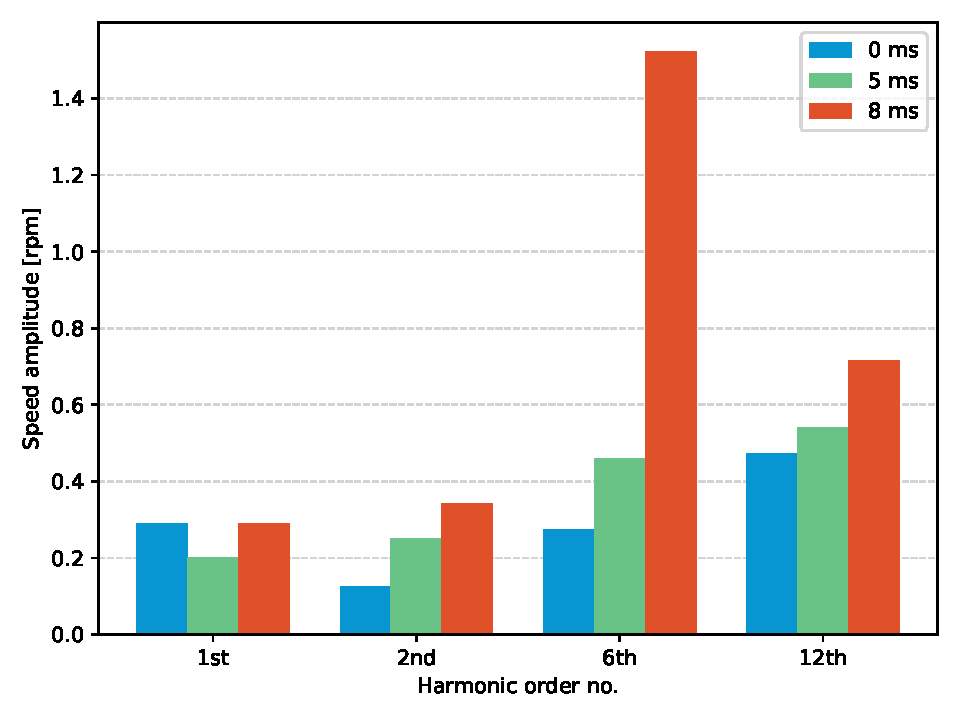
\includegraphics[width=0.8\textwidth]{images/ILC-speed-filters.pdf}
    \caption{ILC based compensation with different speed filtering time constants}
    \label{Fig:ILC-filtering} 
\end{figure}
The forgetting factor solves the noise issue without introducing additional phase shift. Therefore, the forgetting factor cannot amplify pulsations in any circumstances. However, the use of forgetting factor is still a tradeoff. Forgetting factor makes it impossible to achieve perfect compensation \cite{ILC:2004, ILC:2005}. Therefore, as small $\alpha$ value should be used as possible. It was found experimentally that use of the forgetting factor yields better results with noisy motor setup than heavy filtering.

\subsection{Compensation at various speeds}
Figure \ref{fig:compensation-various-speeds} shows compensation performance at different low speeds. Near $60$ rpm speed, both compensators reduce speed pulsations tremendously. When moving to higher speeds, ILC seems to have troubles compensating pulsations and it can be even seen to degrade the performance. The Q-learning based compensator is able to compensate in all operating points, although the performance gets worse at higher speeds. Therefore, The Q-learning based method can be better if the machine is run at various low speed operating points.

However, the compensation is not really important at higher speeds, since pulsations do get reduced automatically due to inertia, as can be seen from the Fig. \ref{fig:compensation-various-speeds}. The pulsations become smaller even with conventional PI speed control when speed is increased. Therefore, ILC is still totally valid compensation method and the compensators should be used only at low speeds where torque pulsations are truly problematic.
\begin{figure}[htb] 
    \centering
    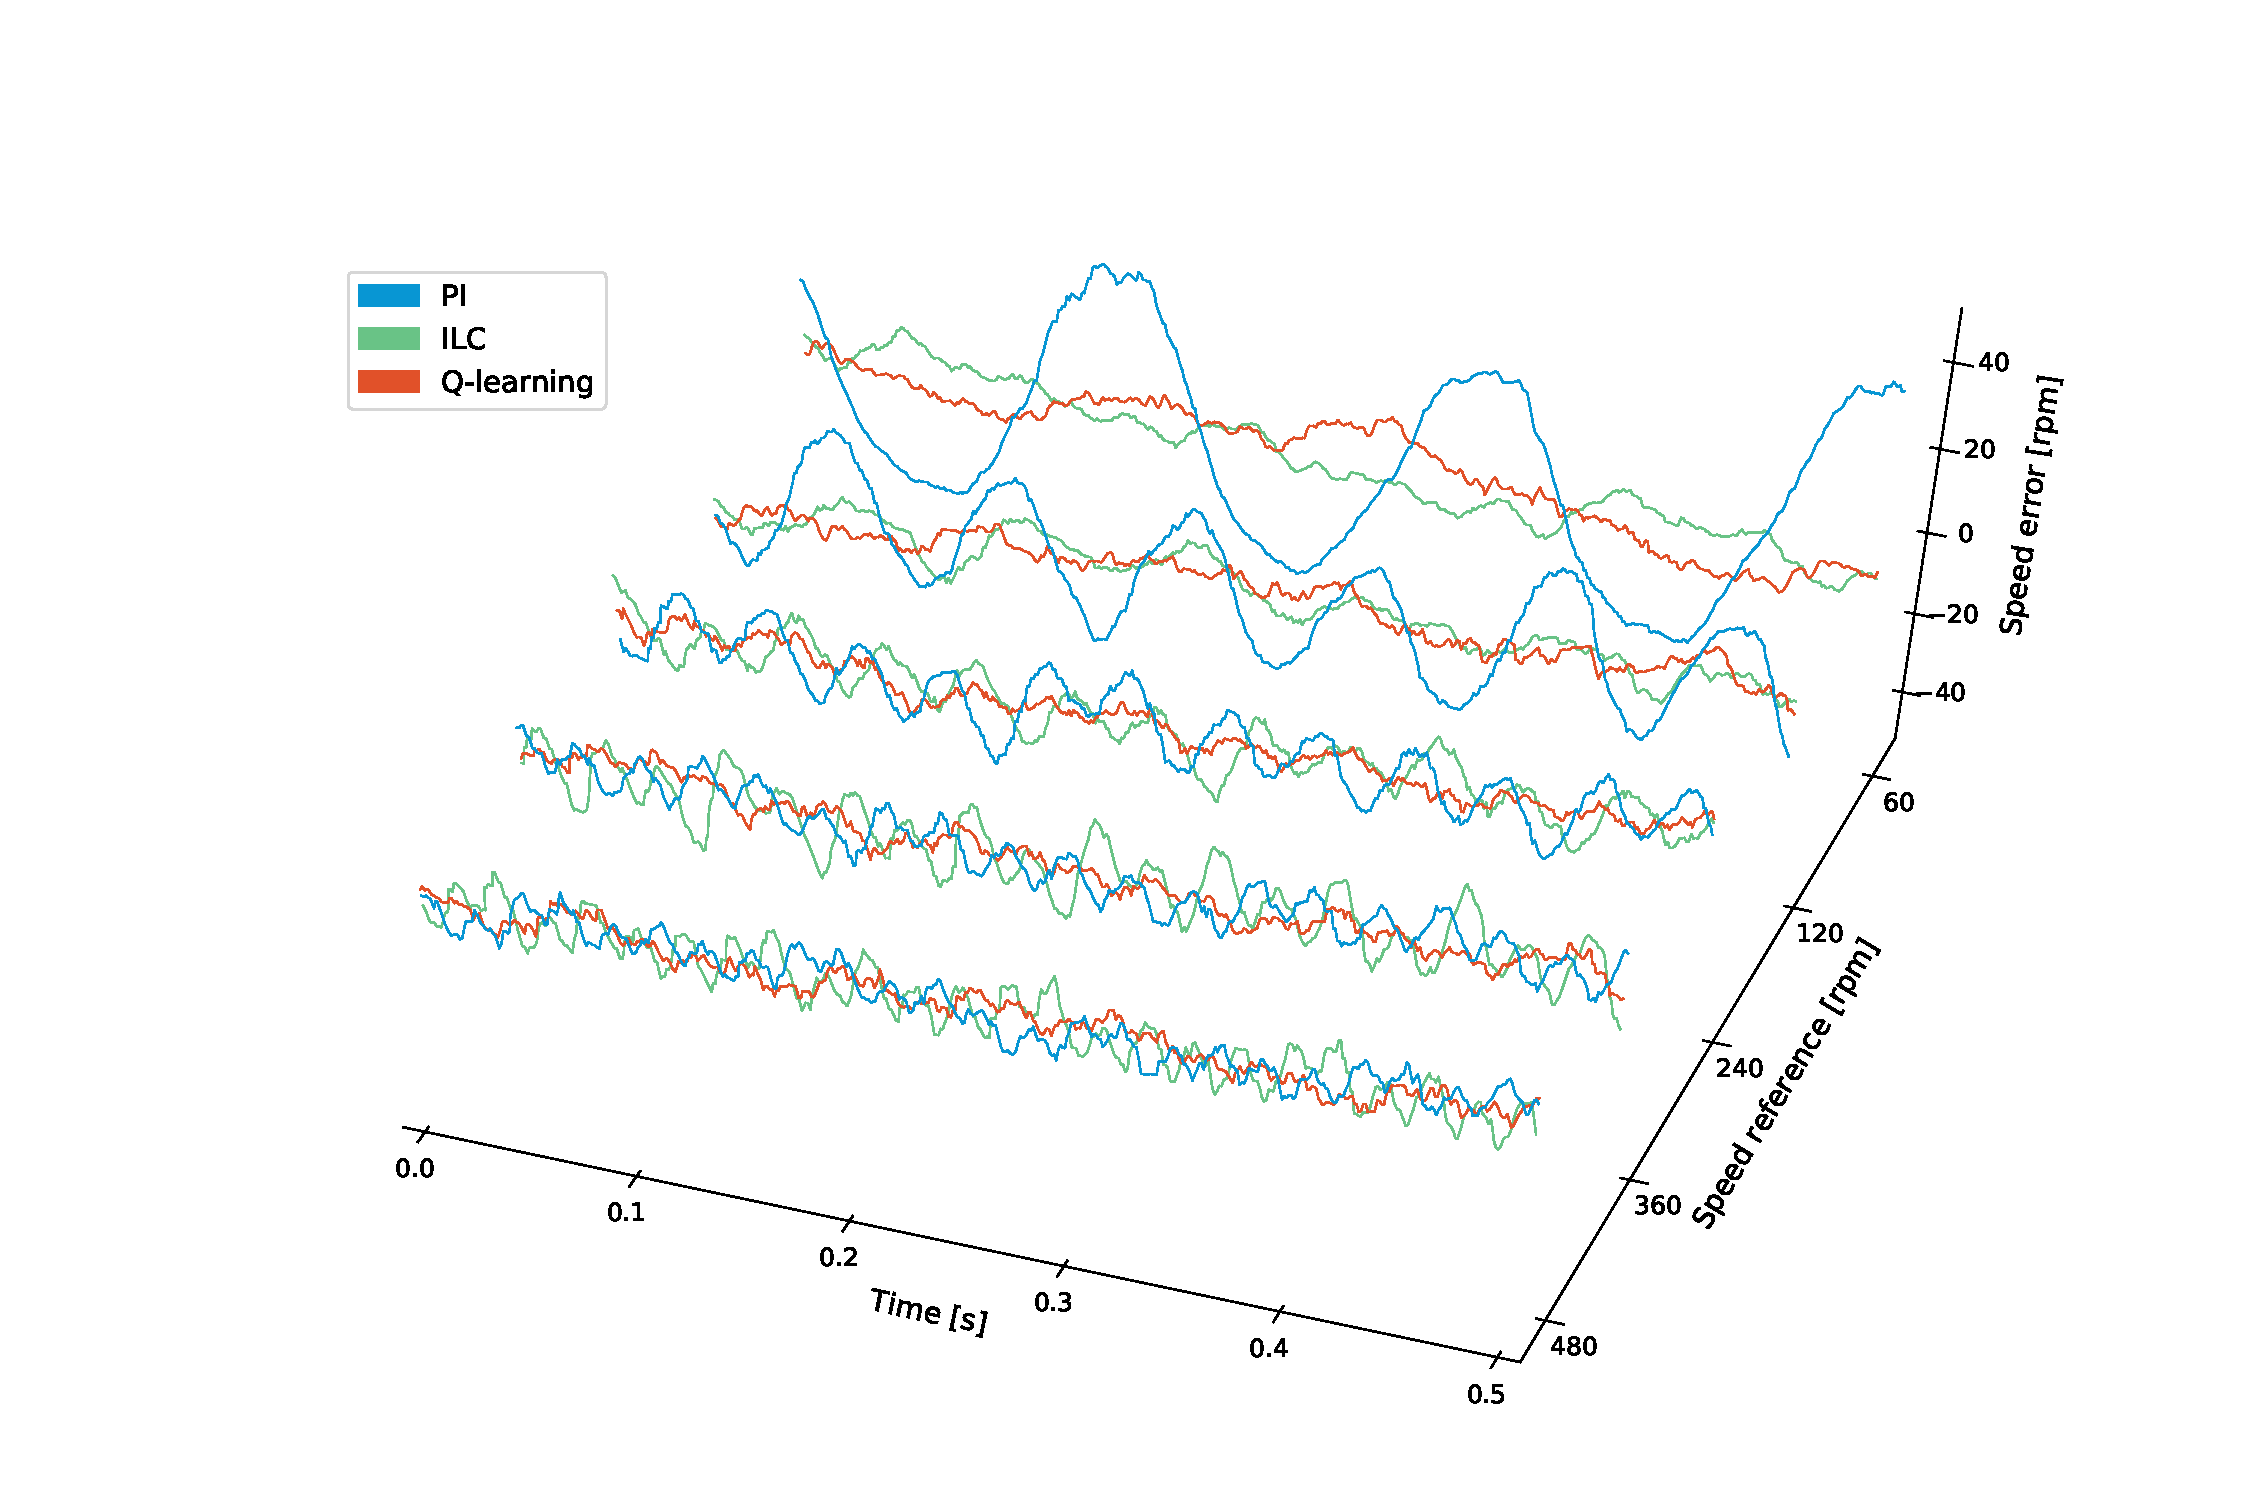
\includegraphics[width=1.0\linewidth]{images/3d-sdm251-pulsation-compensation.pdf} 
    \caption{Speed pulsations getting reduced in different speeds with the servomotor}
    \label{fig:compensation-various-speeds}
\end{figure}

It was found that compensation performance of the Q-learning method is better at high speeds, if lower rotation speed is used for training and the speed is increased after training. This observation can be explained with state skips that occur at high speeds. Due to fast rotation speed, not all states are visited and reduced amount of Q-values are updated. With lower rotation speed, no such skipping occurs. The point where speeds starts to have effect on learning, depends on the number of states and the algorithm update frequency. For example, with $100$ states the rotor should always rotate less than $0.01 \cdot 2\pi \approx 0.06$ rad during single iteration in order to not jump over states. If algorithm is updated every $500 \mu s$, then the speed should stay lower than $120$ rpm during training.

\clearpage
